 \chapter{DUT Development} \label{chap:dut-dev}
 
This chapter describes how to interface the DUT (Design Under Test) a.k.a victim, to the DUT Wrapper.
The DUT Wrapper is included with FOBOS. However, the  DUT is user provided.
The DUT Wrapper handels communication to the Control Board and includes FIFOs to store input data for the DUT along with output FIFO.

\section{Data Flow Description}

Test vectors are sent form PC one at a time to the Control Board which stores them briefly in a FIFO.
The PC sends a command indicating test vector is complete. This will initiates the process of sending the data from the Control Board to the DUT through the interface shown in the figure above.
The DUT wrapper then puts data in the correct FIFOs (PDI, SDI and RDI).
Once the DUT wrapper receives the start command from the controller, it de-assersts the reset signal and the DUT will run and use the data in the FIFOs. The output from the DUT is stored in the DO FIFO.
Once the DO FIFO accumulates EXPECTED\_OUTPUT bytes, the DUT wrapper will send this data to the control board which forwards it to the PC.
This process repeats unitl all traces have been collected.

\begin{center}

\begin{figure}
  \label{fig:fobos-capture}
  \caption{FOBOS Hardware}
  \centering
   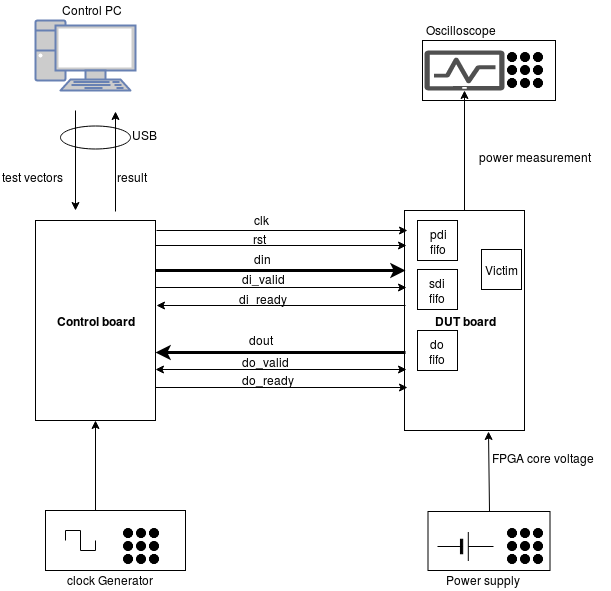
\includegraphics[scale=0.6]{../figures/FOBOS_Capture}
\end{figure}
\end{center}

\section{The DUT Wrapper - DUT interface}

The protocol follows AXI stream protocol.
The DUT (victim) is instantiated as follows in the FOBOS\_DUT.vhd file.
The following is an example of how the DUT is instantiated:

\begin{verbatim}
victim: entity work.victim(behav)
   -- Choices for W and SW are independently any multiple of 4, defined in generics above

   generic map  (
      G_W   => W, -- pdi and do width (mulltiple of 4)
      G_SW  => SW -- sdi width (multiple of 4) 
   )
   port map(
      clk => clk,
      rst => start,  --! The FOBOS_DUT start signal meets requirements for 
      --synchronous resets used in 
      --! CAESAR HW Development Package AEAD
      --data signals
      pdi_data  => pdi_data,
      pdi_valid => pdi_valid,
      pdi_ready => pdi_ready,

      sdi_data => sdi_data,
      sdi_valid => sdi_valid,
      sdi_ready => sdi_ready,
      do_data => result_data,
      do_ready => result_ready,
      do_valid => result_valid

--! if rdi_interface for side-channel protected versions is 
--- required, uncomment the rdi interface
--    ,rdi_data => rdi_data,
--    rdi_ready => rdi_ready,
--    rdi_valid => rdi_valid
);
\end{verbatim}

There are four interfaces for four types of data that can be sent to the DUT:
\begin{enumerate}
 \item Public Data Input (PDI): This is the data that the DUT will process. For example if the DUT is performing encryption, PDI will transfer plaintext.
 \item Secret Data Input (SDI): Secret data interface. For example, encryption keys.
 \item Random Data Input (RDI): Random data interface. This can be used when running protected ciphers that use masking.
 \item Data Out (DO): Output data from the DUT. For example this can be ciphertext.
\end{enumerate}


The generic W corresponds to the PDI and DO width in bits.
The generic SW corresponds to the SDI width in bits.


It is highly recommended that the DUT is tested using the \texttt{sources/dut/fobos\_dut\_tb.vhd} test bench and ensure that the result data in the \texttt{do} port is correct. 
This testbench needs one test vector to be stored in the file \texttt{dinFile.txt} (See Chapter~ \ref{chap:fobos-tv-gen} for information about test-vector generation).